\documentclass{article}
\usepackage{tikz}

\begin{document}
\begin{abstract}
    This is a test.
\end{abstract}
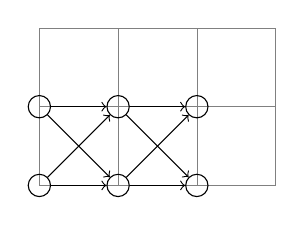
\begin{tikzpicture}
    \draw[help lines] (0,0) grid (3,2);
    \foreach \x in {0,1,2}
    \foreach \y in {0,1}
    \node[draw, circle, inner sep=1mm] (n\x\y) at (\x, \y) {};
    \foreach \x in {0,1}
    \foreach \y in {0,1}
    \foreach \z in {0,1}
    \draw[->] (n\x\y) -- (n\the\numexpr\x+1\relax\z);
\end{tikzpicture}
\end{document}